\documentclass[10pt]{beamer}
\usetheme{jambro}

\title[]{Pensamento Econômico Contemporâneo - Escola novo-Keynesiana}
\author[]{Paulo Victor da Fonseca}
\date{}

\hypersetup{
    colorlinks = true,
    urlcolor = teal,
    linkcolor = teal    
}
\usepackage[portuguese]{babel}
\usepackage{subfig}
%\usepackage{emoji}
\usepackage{amssymb}
\setbeamercovered{transparent}

\begin{document}

\begin{frame}[plain]
    \titlepage{
        \begin{center}
            \begin{minipage}{0.8\textwidth}
                \centering
            \end{minipage}
        \end{center}}
\end{frame}

\begin{frame}{Sumário}
    \tableofcontents
\end{frame}

\section{Introdução}
\begin{frame}{Introdução}
    \begin{itemize}
        \item Principais proposições do Keynesianismo ortodoxo:\bigskip
        \begin{enumerate}
            \item uma economia de mercado não regulamentada apresentará períodos prolongados de excesso de oferta de produto e trabalho ($\neq$ lei de Say) - i.e., economias de mercado apresentarão desemprego involuntário \bigskip
            \item instabilidade agregada (ciclos econômicos) é causado, primordialmente, por distúrbios de demanda agregada\bigskip
            \item a moeda importa, na maior parte do tempo, mas em períodos de recessão profunda a política monetária pode ser ineficaz (Blanchard, 1990a; Krugman, 1998)\bigskip
            \item intervenções governamentais sob a forma de políticas de estabilização têm o potencial de melhorar o bem-estar social e a estabilidade macro
        \end{enumerate}
    \end{itemize}
\end{frame}

\begin{frame}{Introdução}
    \begin{figure}
        \centering
        
\includegraphics[width=0.8\textwidth]{./figures/aula15_fig1.PNG}
        \caption{Freshwater $\times$ saltwater economics.}
        \label{fig1}
    \end{figure}
\end{frame}

\begin{frame}{Introdução}
    \begin{itemize}
        \item Novos-Keynesianos compartilham das proposições do Keynesianismo ortodoxo, mas modelos novo-Keynesianos são diferentes em muitos aspectos\bigskip
        \item Modelos novo-Keynesianos compartilham duas das premissas metodológicas novo-clássica:\bigskip
        \begin{enumerate}
            \item Teorias macroeconômicas requerem fundamentos microeconômicos sólidos\bigskip
            \item Modelos macroeconômicos construídos no arcabouço de equilíbrio geral.
        \end{enumerate}
        \item Microfundamentos RBC: informação perfeita, competição perfeita, ausência de custos de transação, existência de um conjunto completo de mercados\bigskip
        \item Abordagem novo-Keynesiana reconhece importância de uma variedade de imperfeições, e.g.: informação assimétrica, agentes heterogêneos e mercados imperfeitos e incompletos\bigskip
        \item Agenda de pesquisa com objetivo de retificar falhas teóricas do lado de oferta do modelo Keynesiano ortodoxo - reconstrução dos microfundamentos usando teoria microeconômica moderna\bigskip
        \item As imperfeições incorporadas implicarão que oferta agregada responde a variações de demanda agregada
    \end{itemize}
\end{frame}    

\begin{frame}{Introdução}
    \begin{itemize}
        \item Modelos de tradição clássica: hipótese de equilíbrio contínuo de mercado implica que economia não pode ser restrita por deficiência de demanda agregada\bigskip
        
        \item Modelos Keynesianos: ausência de equilíbrio contínuo de mercados - preços não se ajustam rápido o suficiente para equilibrar mercados e, então, choques de oferta e demanda levam a efeitos reais significativos em produto e emprego\bigskip
        \item Keynesianos ortodoxos $\times$ novos-Keynesianos\bigskip
        \item Portanto, novos-Keynesianos tem como objetivo desenvolver uma teoria coerente de oferta agregada onde rigidezes de preços e salários podem ser racionalizadas:\bigskip
        
        \NB{search for rigorous and convincing models of wage and/or price stickiness based on maximising behaviour and rational expectations

            \flushright{(Gordon, 1990)}}
    \end{itemize}
\end{frame}

\begin{frame}{Introdução}
    \begin{itemize}
        \item Novos-Keynesianos: grupo heterogêneo\bigskip
        \item Gregory Mankiw, Lawrence Summers, Olivier Blanchard, Stanley Fischer, Bruce Greenwald, Edmund Phelps, Joseph Stiglitz, Ben Bernanke, Laurence Ball, George Akerlof, Janet Yellen, David Romer, Robert Hall, John Taylor, Dennis Snower, Assar Lindbeck\bigskip
        \item Europeus: Richard Layard, Stephen Nickell, Richard Jackman, Wendy Carlin, David Soskice\bigskip
        \item Europeus: competição imperfeito no mercado de trabalho e no mercado de bens, refletindo elevadas taxas de sindicalização que caracterizam países europeus
    \end{itemize}
\end{frame}

\begin{frame}{Introdução}
    \begin{itemize}
        \item Explicações (mainstream) alternativas do ciclo econômico do começo dos anos 1980s:\bigskip
        \begin{enumerate}
            \item teorias novo-clássicas de preços flexíveis e percepções monetárias errôneas de Lucas\bigskip
            \item modelos expectacionais de preços rígidos enfatizando algum elemento de rigidez de salários e preços (Fischer, 1977; Phelps e Taylor, 1977; Taylor, 1980)\bigskip
            \item teoria RBC
        \end{enumerate}
    \end{itemize}
\end{frame}

\begin{frame}{Economia novo-Keynesiana}
    \begin{itemize}
        \item Mankiw e Romer (1991):
        \begin{enumerate}
            \item A teoria viola a dicotomia clássica? Isto é, a moeda é não-neutra?\bigskip
            \item A teoria assume que imperfeições reais de mercado são cruciais para a compreensão das flutuações econômicas?\bigskip
        \end{enumerate}
        \item Escola novo-Keynesiana: resposta afirmativa para ambas as perguntas\bigskip
        \item Não-neutralidade emerge da rigidez de preços, imperfeições de mercado explicam este comportamento dos preços\bigskip
        \item A interação entre imperfeições reais e nominais distinguem a economia novo-Keynesiana (Mankiw e Romer, 1991)
    \end{itemize}    
\end{frame}

\begin{frame}{Economia novo-Keynesiana}
    \begin{itemize}
        \item Novos-Keynesianos não são protagonistas no debate Keynesianos-monetaristas da década de 1960:\bigskip
        \begin{enumerate}
            \item Não há uma visão unificada sobre o papel da política fiscal - novos-Keynesianos dão um peso muito maior sobre o papel estabilizador da política monetária (nova economia monetária)\bigskip
            \item Não há uma visão unificada acerca da desejabilidade e viabilidade de políticas ativistas (discricionárias) de estabilização
        \end{enumerate}
    \end{itemize}
\end{frame}

\begin{frame}{Economia novo-Keynesiana}
    \begin{itemize}
        \item Algumas características:\bigskip
        \begin{enumerate}
            \item Em contraste com modelos novo-clássicos habitados por agentes tomadores de preços, modelos novo-Keynesianos assumem firmas fixadoras de preços em um ambiente de competição monopolística (Robinson, 1933; Chamberlin, 1933)\bigskip
            \item A maioria dos modelos novo-Keynesianos assume que expectativas são formadas racionalmente (alguns permanecem críticos com relação aos fundamentos teóricos e suporte empírico da HER)\bigskip
            \item Choques de demanda e oferta como potenciais fontes de instabilidade (Blanchard e Quah, 1989)\bigskip
            \item Muitos (não todos) compartilham a visão Keynesiana de que desemprego involuntário é possível e provável\bigskip
        \end{enumerate}
    \end{itemize}
\end{frame}

\begin{frame}{Economia novo-Keynesiana}
    \begin{itemize}
        \item Grande heterogeneidade entre novos-Keynesianos: conveniente dividir as explicações de rigidezes entre aquelas que focam em rigidezes nominais e as que focam em rigidezes reais\bigskip
        \item Rigidez nominal: quando algo impede o ajuste perfeito do nível geral de preços frente a distúrbios de demanda nominal\bigskip
        \item Rigidez real: algum fator impede ajuste de salários reais ou se há alguma rigidez de um salário relativo a outro, ou de um preço relativo a outro
    \end{itemize}
\end{frame}

\section{Rigidezes nominais}
\begin{frame}{Rigidez nominal}
    \begin{itemize}
        \item Em linha com a abordagem de teoria da escolha da análise novo-clássica, a abordagem NK assume que trabalhadores e firmas são maximizadores de utilidade e lucros, respectivamente\bigskip
        \item Novos-clássicos: modelo de leilões de preços flexíveis adotado e aplicado à análise das transações realizadas em todos os mercados (incluindo mercado de trabalho)\bigskip
        \item Novos-Keynesianos: distinção entre mercados que são essencialmente de preços fixos (predominantemente o mercado de trabalho e boa parte dos mercados de bens) e mercados de preços flexíveis (mercados financeiros e de commodities)\bigskip
        \item Mercados de preços fixos: a norma é fixação de preços, com inércia de preços e salários uma realidade\bigskip
        \item Não-neutralidade monetária é gerada pela incapacidade de preços e salários de se ajustar instantaneamente ao novo nível de equilíbrio de mercado após um choque de demanda agregada
    \end{itemize}
\end{frame}

\begin{frame}{Rigidez nominal}
    \begin{itemize}
        \item Keynesianos tradicionalmente concentraram-se no mercado de trabalho e em rigidezes de salário nominal\bigskip
        \item No entanto, é importante observar que para qualquer dada trajetória de demanda agregada nominal, é a rigidez de preços, e não de salários, que é necessária para gerar flutuações no produto agregado real\bigskip
        \item Mas a `primeira onda' de modelos novo-Keynesianos focou em rigidez de salários nominais
    \end{itemize}
\end{frame}

\begin{frame}{Rigidez de salário nominal}
    \begin{itemize}
        \item Modelo Keynesiano tradicional: nível de preços impedido de cair para restaurar equilíbrio pela incapacidade de salários nominais (custos) em se ajustarem - Figura \ref{fig2}\bigskip
        \item Modelos novo-clássicos: choques antecipados de política monetária levam a uma redução imediata de salários nominais e preços para valor de equilíbrio, mantendo produto e emprego agregados\bigskip
        \item Ineficácia de política monetária: resultado da hipótese de expectativas racionais\bigskip
        \item Fischer (1977) e Phelps e Taylor (1977): choques nominais produzem efeitos reais em modelos com HER se a hipótese de equilíbrio contínuo de mercado for abandonada\bigskip
        \item \hlight{Hipótese de expectativas racionais não implica o fim da economia Keynesiana}
    \end{itemize}
\end{frame}

\begin{frame}{Rigidez de salário nominal}
    \begin{figure}
        \centering
        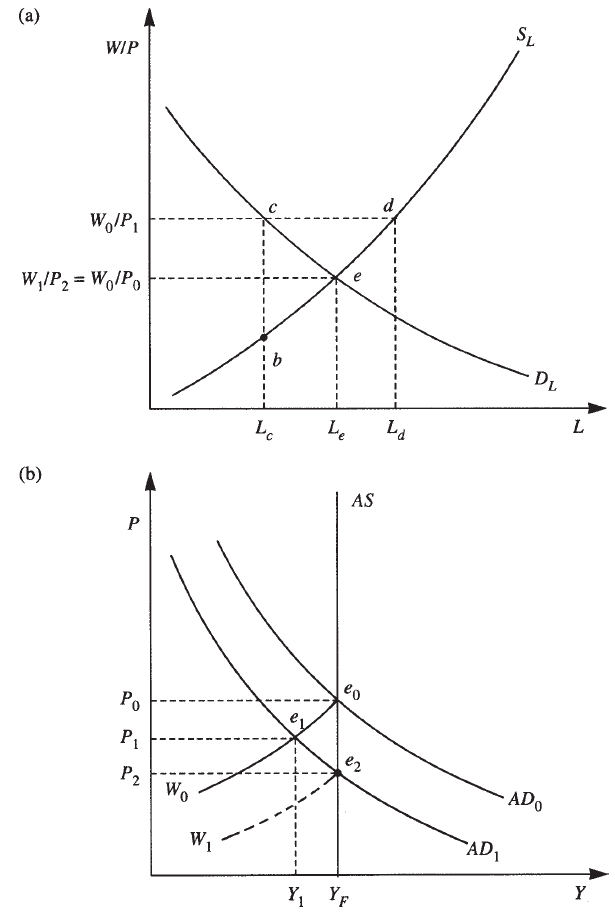
\includegraphics[width=0.3\textwidth]{./figures/aula5_fig1.PNG}
        \caption{Desemprego involuntário - modelo Keynesiano tradicional.}
        \label{fig2}
    \end{figure}
\end{frame}

\begin{frame}{Rigidez de salário nominal}
    \begin{itemize}
        \item Fischer (1977) e Taylor (1980): introdução de inércia nominal sob a forma de contratos salariais de longo prazo\bigskip
        \item Salários não são determinados em mercados à vista (spot markets) mas tendem a ser fixados por um período de tempo acordado sob a forma de um contrato explícito (ou implícito)\bigskip
        \item A existência de contratos de longo prazo pode gerar suficiente rigidez de salário nominal para que política monetária reestabeleça sua efetividade\bigskip
        \item Note, no entanto, que nem Fischer nem Phelps e Taylor forneceram um microfundamento rigoroso para as hipóteses de fixação de preços e salários\bigskip
        \item Ao invés disso, há uma ``preferência revelada'' por contratos salariais de longo prazo refletindo as desvantagens percebidas de incorrer em ajustes frequentes de preços e salários
    \end{itemize}
\end{frame}

\begin{frame}{Rigidez de salário nominal}
    \begin{itemize}
        \item Fischer: modelo com estrutura similar ao de Lucas-Sargent-Wallace\bigskip
        \item Função de oferta agregada de Lucas:
        \begin{equation}
            Y_t = Y_t^n + \alpha(\dot{P}_t - \dot{P}_t^e), \qquad \alpha > 0
        \end{equation}
        \item Com expectativas formadas racionalmente:
        \begin{equation}
            Y_t = Y_t^n + \alpha\left[\dot{P}_t - \mathbb{E}(\dot{P}_t|\Omega_{t-1})\right]
        \end{equation}
        \item Modelo assume que não há crescimento, portanto, assume-se que negociadores salariais buscam constância de salário real fixando aumentos de salários nominais iguais à expectativa inflacionária:
        \begin{equation}
            \dot{W}_t = \mathbb{E}(\dot{P}_t|\Omega_{t-1})
        \end{equation}
    \end{itemize}
\end{frame}

\begin{frame}{Rigidez de salário nominal}
    \begin{itemize}
        \item Portanto, oferta agregada é uma função inversa do salário real (\hlight{salário real é contracíclico}):
        \begin{equation}
            Y_t = Y_t^n + \alpha[\dot{P}_t - \dot{W}_t] 
        \end{equation}
        \item Para o contratos multi-períodos, aumentos dos salários nominais são fixados em $\dot{W}_t = \dot{W}_t^*$\bigskip
        \item Fischer (1977) assume (`hipótese empiricamente razoável') que agentes econômicos negociam salários em termos nominais para períodos mais longos do que o tempo que leva para a autoridade monetária reagir ao ambiente econômico\bigskip
        \item Como autoridades monetárias podem alterar a oferta de moeda (e, portanto, inflação) de maneira mais frequente que contratos de trabalho sobrepostos são renegociados, a política monetária pode ter efeitos reais no curto prazo (mantendo-se neutra no longo prazo)
    \end{itemize}
\end{frame}

\begin{frame}{Rigidez de salário nominal}
    \begin{figure}
        \centering
        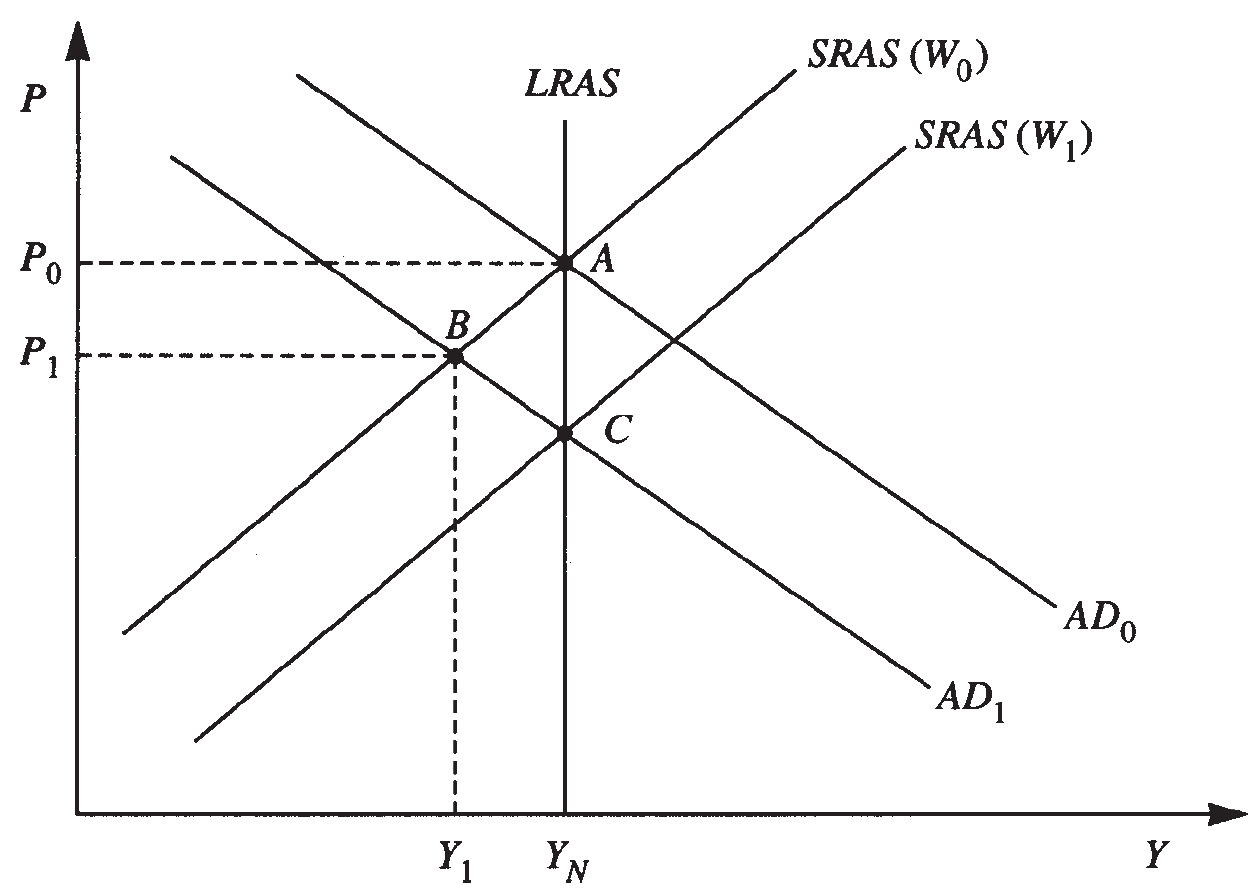
\includegraphics[width=0.6\textwidth]{./figures/aula15_fig2.PNG}
        \caption{Contratos de salários nominais, expectativas racionais e política monetária. Fonte: Snowdon e Vane (2005).}
        \label{fig3}
    \end{figure}
\end{frame}

\begin{frame}{Rigidez de salário nominal}
    \begin{itemize}
        \item Economia operando ponto A\bigskip
        \item Suponha um choque não-antecipado de demanda agregada (e.g., queda na velocidade) - desloca curva de $AD_0$ para $AD_1$\bigskip
        \item Se preços são flexíveis mas salários nominais temporariamente rígidos (fixados em $W_0$) como resultado dos contratos negociados no período anterior que se estendem para além do período corrente, então a economia se move para o ponto B (produto agregado real contrai de $Y_N$ para $Y_1$)\bigskip
        \item Se preços e salários são flexíveis, curva de OA de curto prazo deslocaria para a direita - $SRAS(W_0)$ para $SRAS(W_1)$, reestabelecendo produto natural ponto C\bigskip
        \item A existência de contratos salariais nominais de longo prazo impedem que isso aconteça e dá oportunidade para que autoridade monetária expanda a oferta de moeda que, mesmo que antecipado, desloca DA para a direita reestabelecendo equilíbrio no ponto A
    \end{itemize}
\end{frame}

\begin{frame}{Rigidez de salário nominal}
    \begin{itemize}
        \item Caso autoridades consigam reagir a choques exógenos numa frequência maior que setor privado possa renegociar salários nominais há espaço para gerenciamento de DA para estabilizar a economia (mesmo que agentes formem expectativas racionalmente)\bigskip
        \item A não-neutralidade da moeda no modelo de Fischer não se deve a uma surpresa monetária não-antecipada\bigskip
        \item Políticas monetárias antecipadas têm efeitos reais porque são baseadas em informações que só se tornam disponíveis depois que o contrato foi firmado
    \end{itemize}
\end{frame}

\begin{frame}{Rigidez de salário nominal}
    \begin{itemize}
        \item Contratos salariais são características importante em quase todas economias desenvolvidas: heterogeneidade com relação à duração de contratos e timing de renegociação\bigskip
        \item Japão: contratos de salários nominais tipicamente duram 1 ano e expiram simultaneamente. Renegociações sincronizadas (sistema \emph{shunto}) é consistente com maior estabilidade macro do que em países que apresentam contratos não-sincronizados (sobrepostos)\bigskip
        \item EUA: contratos sobrepostos/não-sincronizados tipicamente de 3 anos (Gordon, 1982b; Hall e Taylor, 1997)\bigskip
        \item UK: contratos não-sincronizados com duração de 1 ano
    \end{itemize}
\end{frame}

\begin{frame}{Rigidez de salário nominal}
    \begin{itemize}
        \item Com contratos sobrepostos, salários nominais exibirão mais inércia frente a choques do que seria o caso com renegociações sincronizadas\bigskip
        \item Taylor (1980): se trabalhadores estão preocupados com seus salários nominais relativos a outros, então, contratos sobrepostos permitirão que os impactos da política monetária sobre variáveis reais persistam por um tempo bem maior do que a extensão do período de contrato\bigskip
        \item Taylor (1992b): a responsividade de salários a choques de oferta e demanda é maior no Japão que nos EUA, Canadá e outros países europeus, e isso possibilitou uma maior estabilidade macro no Japão durante os anos 1970s e 1980s
    \end{itemize}
\end{frame}

\begin{frame}{Rigidez de salário nominal}
    \begin{itemize}
        \item Por que contratos de longo prazo são formados se aumentam instabilidade macro? Phelps (1985, 1990) argumenta que há razões privadas para firmas e trabalhadores:\bigskip
        \begin{enumerate}
            \item Negociações salariais são custosas para firmas e trabalhadores: pesquisas com relação à estrutura de relatividades dentro e fora da organização; necessidade de formar previsões p/ variáveis relevantes (produtividade, inflação, demanda, lucros e preços). Quanto maior o período do contrato, menos frequentemente estes custos de transação serão incorridos\bigskip
            \item Sempre existe potencial para não haver um acordo: trabalhadores podem recorrer a greves para reforçar posição no processo de barganha (disrupções custosas tanto para firmas quanto trabalhadores)\bigskip
            \item Não será uma estratégia ótima para uma firma ajustar seus salários para o novo valor de equilíbrio frente a um choque adverso de demanda porque, caso outras firmas não o façam, a firma reduziria seu salário relativo e isso, por sua vez, poderia aumentar a rotatividade do trabalho
        \end{enumerate}
    \end{itemize}
\end{frame}

\begin{frame}{Rigidez de salário nominal}
    \begin{itemize}
        \item Por que contratos salariais não são indexados à taxa de inflação?\bigskip
        \item Acordos completos de custo de vida (COLAs) são arriscados para as firmas pois nem todos os choques são choques de demanda nominal\bigskip
        \item Se uma firma indexa seus salários à inflação então, choques de oferta (como os dos anos 1970s) levariam a um aumento no nível de preços e, com isso, a um aumento nos custos salariais das firmas e, portanto, impedindo a queda necessária de salário real implicada por um choque de energia
    \end{itemize}
\end{frame}

\begin{frame}{Rigidez de salário nominal}
    \begin{itemize}
        \item Contratos salariais não-sincronizados também podem ter propósitos microeconômicos, mesmo que causem instabilidade macro\bigskip
        \item Se firmas tem informação imperfeita a respeito da situação econômica corrente, podem obter informações relevantes ao observar preços e salários fixados por outras firmas\bigskip
        \item Hall e Taylor (1997): fixação sobrepostas de salários provê informações úteis para firmas e trabalhadores a respeito de variações na estrutura de preços e salários\bigskip
        \item Em um sistema decentralizado sem acordos sobrepostos, observaríamos uma enorme variabilidade introduzida no sistema\bigskip
        \item Ball e Cecchetti (1988): informação imperfeita pode tornar estratégias de salários e preços sobrepostos socialmente ótimos ao ajudar firmas a fixar preços próximo aos níveis de informação perfeita, levando a ganhos de eficiência que mais que compensam os custos de inércia no nível de preços\bigskip
        \item \hlight{Ajustes salariais sobrepostos podem emergir do comportamento racional dos agentes. Fixação de salários em um sistema sincronizado parece requerer algum grau de participação ativa do governo} 
    \end{itemize}
\end{frame}

\begin{frame}{Rigidez nominal de preços}
    \begin{itemize}
        \item Críticas a modelos Keynesianos baseados em rigidez de salários nominais:\bigskip
        \begin{enumerate}
            \item Existência de contratos não é baseada em princípios micro sólidos\bigskip
            \item Comportamento contra-cíclico dos salários reais: modelo de Fischer, uma expansão monetária aumenta emprego agregado ao reduzir salários reais\bigskip
        \end{enumerate}        
    \end{itemize}
    \NB{
        It was thinking about the real wage puzzle that originally got me interested in thinking about imperfections in goods markets, and eventually, about monopolistically competitive firms facing menu consistente

        \flushright{(Mankiw, 1991)}
    }
\end{frame}

\begin{frame}{Rigidez nominal de preços}
    \begin{itemize}
        \item Termo novos-Keynesianos emerge em meados dos 1980s como descrição de novas teorias que visavam dar fundamentos micro mais sólidos para o fenômeno de rigidez nominal de preços\bigskip
        \item A nova ideia fundamental de modelos novos-Keynesianos é a de competição imperfeita\bigskip
        \item Diferenciando novos-Keynesianos de Keynes, Keynesianos ortodoxos, monetaristas e novos-clássicos
    \end{itemize}
\end{frame}

\begin{frame}{Rigidez nominal de preços}
    \begin{itemize}
        \item $\nexists$ custos de ajustamento de preços e o não ajustamento de preços envolvesse variações substanciais na lucratividade da firma: grau elevado de flexibilidade de preços\bigskip
        \item Competição perfeita: firma tomadora de preços, preços variam automaticamente com mudanças nas condições de oferta e demanda (firma individual não tem decisão de precificação)\bigskip
        \item Competição imperfeita: lucratividade varia com mudanças no preço da firma porque suas vendas não serão reduzidas a zero caso haja aumento marginal no preço\bigskip
        \item Redução de preços aumenta vendas mas resulta em menos receita por unidade vendida\bigskip
        \item \hlight{Desvios do preço com relação ao nível ótimo resultará apenas em reduções de segunda ordem nos lucros}
    \end{itemize}
\end{frame}

\begin{frame}{Rigidez nominal de preços}
    \begin{itemize}
        \item \hlight{Portanto, presença de pequenos custos de ajustamento nos preços pode gerar rigidez nominal de preços agregada considerável}\bigskip
        \item 'PAYM insight' (Parkin, 1986; Akerlof e Yellen, 1985a; Mankiw, 1985)\bigskip
        \item Custo privado de rigidezes nominais para firma individual é muito menor que as consequências macro destas rigidezes\bigskip
        \item Presença de fricções ou barreiras ao ajustamento de preços (\textcolor{purple}{custos de menu}): custos físicos de redeterminar preços, tempo de gerenciamento para supervisão e renegociação de contratos de compras e vendas com fornecedores e consumidores
    \end{itemize}
\end{frame}

\begin{frame}{Rigidez nominal de preços}
    \begin{itemize}
        \item Competição imperfeita a demanda da firma depende de:\bigskip
        \begin{enumerate}
            \item preço relativo\bigskip
            \item demanda agregada\bigskip
        \end{enumerate}
        \item Suponha queda de DA que faz com que a curva de demanda de uma firma sob competição imperfeita desloque para a esquerda\bigskip
        \item Deslocamento pode reduzir consideravelmente a lucratividade da firma\bigskip
        \item No entanto, ao se deparar com essa nova curva de demanda, firma pode obter ganhos limitados com o ajustamento de preços\bigskip
        \item Dada a nova situação, a firma deve escolher um ponto sobre a nova curva de demanda
    \end{itemize}
\end{frame}
\begin{frame}{Rigidez nominal de preços}
    \begin{figure}
        \centering
        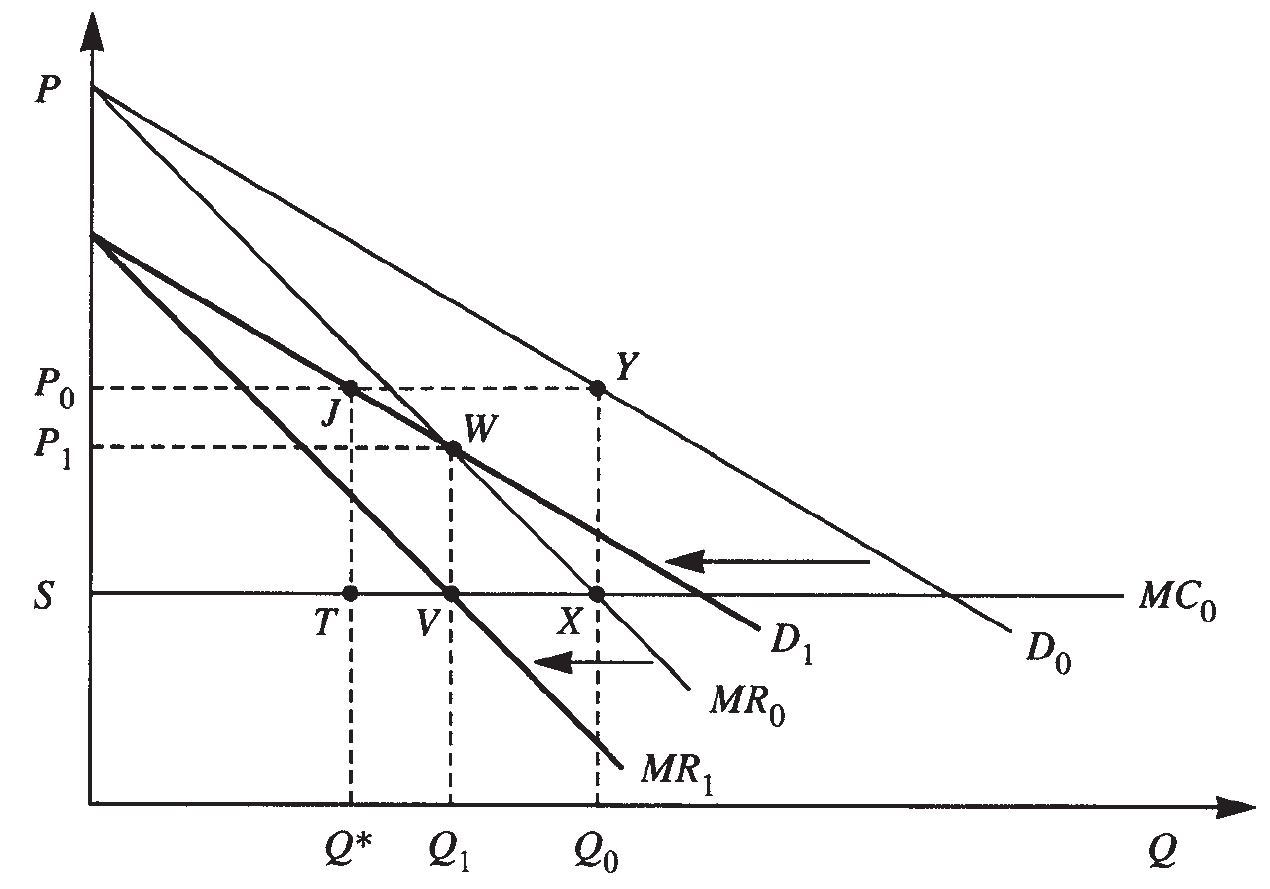
\includegraphics[width=0.6\textwidth]{./figures/aula15_fig3.PNG}
        \caption{Ajustamento de preços sob competição imperfeita. Fonte: Snowdon e Vane (2005).}
        \label{aula15_fig3}
    \end{figure}
\end{frame}

\begin{frame}{Rigidez nominal de preços}
    \begin{itemize}
        \item Hipótese: custo marginal não varia com produção  no intervalo analisado\bigskip
        \item Antes do deslocamento de demanda, lucratividade: $SP_0YX$\bigskip
        \item Como firma é fixadora de preços, deve decidir se reduz preço para o novo nível ótimo ou não\bigskip
        \item Após deslocamento de demanda, se firma não ajusta preços: $SP_0JT$\bigskip
        \item Se preço ajustado para novo nível ótimo: $SP_1WV$\bigskip
        \item Se não há custos de ajustamento, firma maximizadora de lucros reduz preços de $P_1$ para $P_0$\bigskip
        \item Se a firma se depara com custos de menu de $z$, firma pode decidir manter preço em $P_0$
    \end{itemize}
\end{frame}

\begin{frame}{Rigidez nominal de preços}
    \begin{figure}
        \centering
        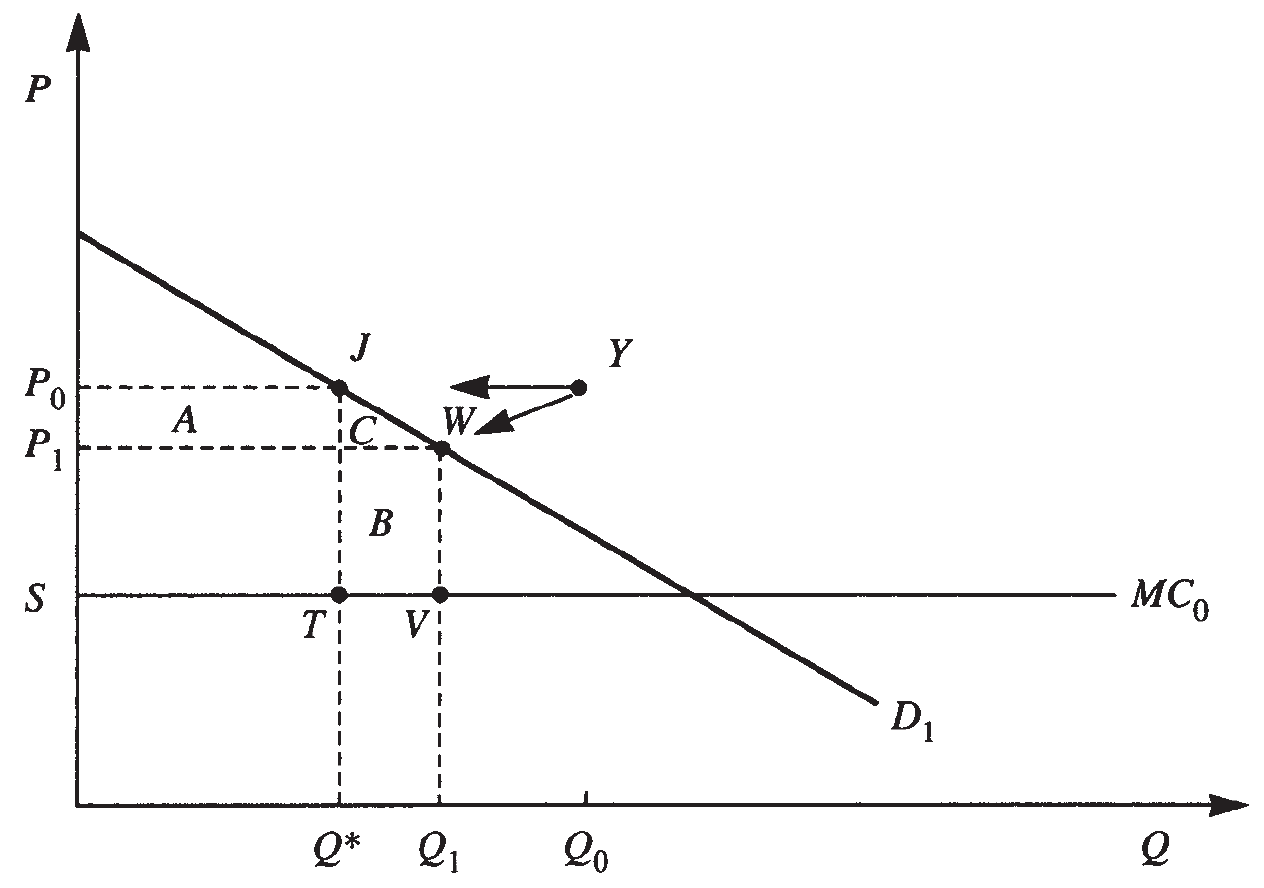
\includegraphics[width=0.6\textwidth]{./figures/aula15_fig4.PNG}
        \caption{Custos de menu $\times$ ajuste de preços. Fonte: Snowdon e Vane (2005).}
        \label{aula15_fig4}
    \end{figure}
\end{frame}

\begin{frame}{Rigidez nominal de preços}
    \begin{itemize}
        \item Ao reduzir preços, firma aumenta lucros em $B - A$\bigskip
        \item Não há incentivos para redução de preços se $z > B - A$\bigskip
        \item Perda social de produzir $Q^*$ ao invés de $Q_1$ é dada por $B + C$, que representa a perda de excedente total\bigskip
        \item Se após a redução de demanda tivermos que $B + C > z > B - A$, então, a firma não reduzirá preços mesmo que seja socialmente ótimo\bigskip
        \item \hlight{Quanto mais plana for a agenda de custo marginal $MC$, menores os custos de menu necessários para validar a decisão da firma de manter preços inalterados}
    \end{itemize}
\end{frame}

\begin{frame}{Rigidez nominal de preços}
    \begin{figure}
        \centering
        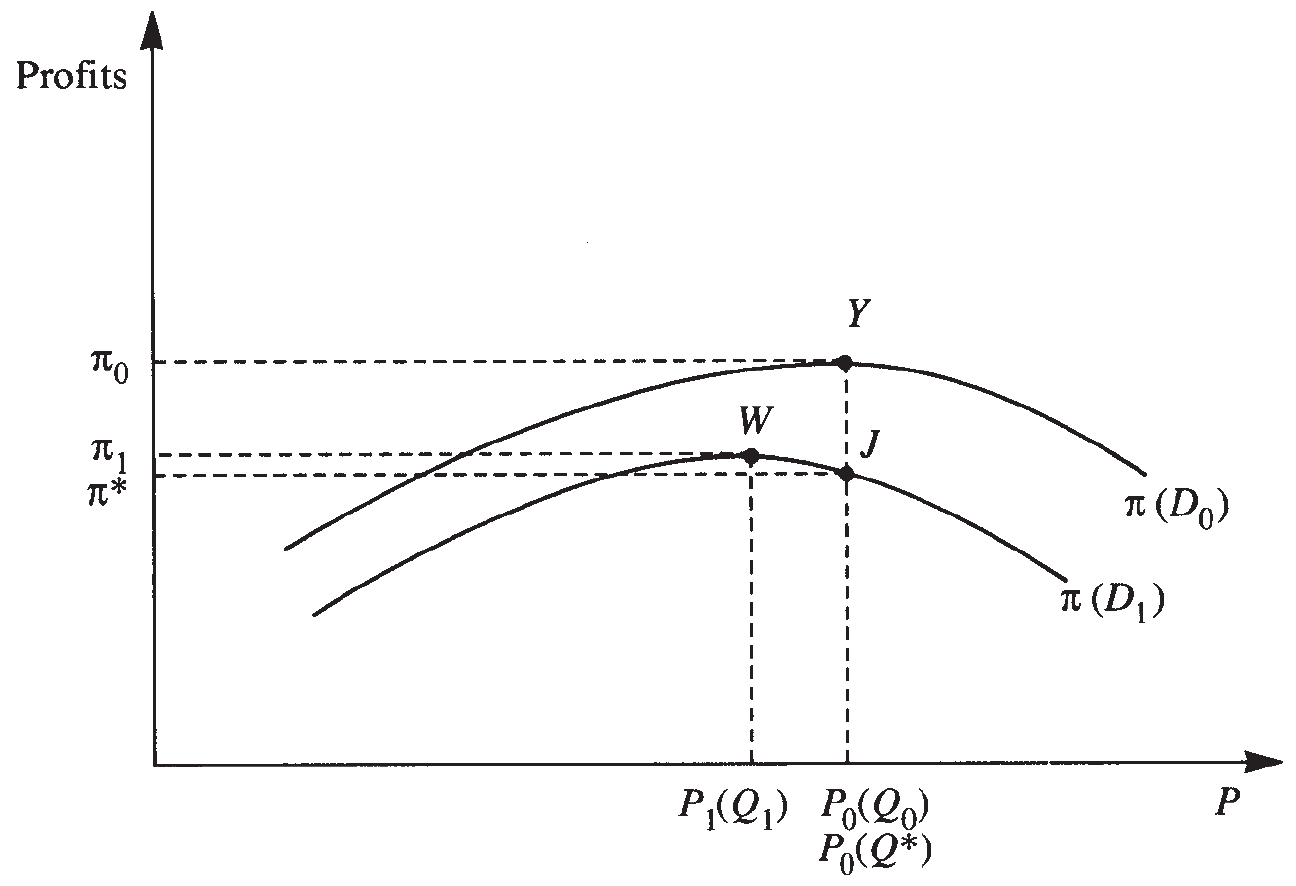
\includegraphics[width=0.6\textwidth]{./figures/aula15_fig5.PNG}
        \caption{Near rationality. Fonte: Snowdon e Vane (2005).}
        \label{aula15_fig5}
    \end{figure}
\end{frame}

\begin{frame}{Rigidez nominal de preços}
    \begin{itemize}
        \item Akerlof e Yellen (1985a, 1985b): comportamento inercial de preços e salários por parte das firmas pode ser `quase racional'\bigskip
        \item Comportamento sub-ótimo de firmas na fixação de preços pode induzir perdas mas que provavelmente serão de segunda ordem: Figura \ref{aula15_fig5}\bigskip
        \item Preço que maximiza lucros após redução de demanda é indicado por $P_1$\bigskip
        \item A redução nos lucros resultante do não ajustamento de preços é $(\pi_1 - \pi^*)$ que é pequeno mesmo se desconsiderarmos custos de menu (na figura anterior: $B - A$ é pequeno)\bigskip
        \item Akerlof e Yellen (1985a) mostram ainda que se competição imperfeita no mercado de bens + salário eficiência no mercado de trabalho, choques de DA levam a flutuações cíclicas
    \end{itemize}
\end{frame}

\begin{frame}{Rigidez nominal de preços}
    \begin{itemize}
        \item A decisão ótima da firma de manter preço em $P_0$, se repetida pelas outras firmas, pode ter efeitos macro significativos\bigskip
        \item Blanchard e Kiyotaki (1987): os efeitos macro de rigidez nominal de preços difere dos custos privados porque rigidez de preços gera uma externalidade de demanda agregada\bigskip
        \item Socialmente preferível se todas as firmas reduzissem preços, mas não existem incentivos individuais para isso\bigskip
        \item Diante de um declínio de DA (que desloca demanda individual) e ausência de custo de menu, todas as firmas reduziriam preços\bigskip
        \item Nesse caso, cada firma perceberia uma redução no custo de seus insumos, inclusive salários nominais
    \end{itemize}
\end{frame}

\begin{frame}{Rigidez nominal de preços}
    \begin{itemize}
        \item A curva de custo marginal de cada firma começa a se deslocar para baixo, o que possibilita novas reduções nos preços\bigskip
        \item Nas figuras anteriores, deslocamentos da curva de custo marginal possibilitam expansão na produção\bigskip
        \item Como todas as firmas incorrem em novas reduções de preços, preços de insumos caem novamente, resultando em nova redução na curva MC\bigskip
        \item Este processo de deflação de preços aumenta valor de encaixes reais o que, por sua vez, reduz taxa de juros e, então, DA aumenta\bigskip
        \item Isso desloca curva de demanda individual para a direita, fazendo com que produção retorne para nível $Q_0$
    \end{itemize}
\end{frame}

\begin{frame}{Rigidez nominal de preços}
    \begin{itemize}
        \item Se custos de menu e/ou quase racionalidade causam rigidez nominal de preços, choques de DA vão causar grandes flutuações no produto e bem-estar\bigskip
        \item Como essas flutuações são ineficientes, há margem para políticas de estabilização\bigskip
        \item Se salários nominais são rígidos (contratos de longo prazo) a curva de MC será viscosa, reforçando o impacto de custos de menu sobre rigidezes de preços
    \end{itemize}
\end{frame}

% \begin{frame}{Rigidez nominal de preços}
%     \begin{itemize}
%         \item 
%     \end{itemize}
% \end{frame}

\section{Rigidez real}
\begin{frame}{Rigidez real}
    \begin{itemize}
        \item Ball et al. (1988) crítica à custos de menu: modelos com fricções nominais podem, em teoria, produzir rigidezes nominais significativas, mas apenas para `valores de parâmetros pouco plausíveis'\bigskip
        \item Ball e Romer (1990): rigidez nominal substancial pode resultar de uma combinação de rigidezes reais e pequenas fricções de ajuste nominal\bigskip
        \item Se todos os preços nominais são perfeitamente flexíveis, choques nominais mantem equilíbrio real inalterado\bigskip
        \item Ball e Romer (1990): rigidez real não implica rigidez nominal - sem uma fonte independente de rigidez nominal, preços se ajustam completamente a choques nominais, independentemente da magnitude das rigidezes reais\bigskip
        \item No entanto, \hlight{rigidez de preços e salários reais amplificam  as não-neutralidades que resultam de pequenas fricções nominais}
    \end{itemize}
\end{frame}

\begin{frame}{Rigidez real}
    \begin{itemize}
        \item Considere o impacto de uma queda na oferta de moeda\bigskip
        \item Suponha que custos de menu impeçam firmas de reduzir preços frente a este choque nominal\bigskip
        \item Portanto, produto real irá declinar\bigskip
        \item Cada firma, sob competição monopolística, notará um deslocamento p/ esquerda de sua curva de demanda\bigskip
        \item Como cada firma está com um nível de produção menor, a demanda efetiva por mão-de-obra cai
    \end{itemize}
\end{frame}

\begin{frame}{Rigidez real}
    \begin{itemize}
        \item Se oferta de mão-de-obra é inelástica, o deslocamento na demanda por trabalho induzirá uma queda significativa nos salários reais (haverá um declínio dos salários nominais)\bigskip
        \item Essa queda do salário real reduz custo marginal, queda que será fortemente reforçada se o produto marginal do trabalho aumentar consideravelmente à medida que o insumo mão-de-obra decai\bigskip
        \item Uma curva de MC positivamente inclinada aumenta significativamente o incentivo para reduzir preços e eliminaria qualquer barreira plausível para ajustes nominais\bigskip
        \item A não ser que a elasticidade da demanda ao preço existente caia à medida que a curva de demanda individual desloca para a esquerda\bigskip
        \item Quanto maior a queda da elasticidade da demanda ao preço existente à medida que a produção cai, mais a curva de receita marginal se deslocará para a esquerda e, portanto, menor o incentivo para que a firma reduza seu preço
    \end{itemize}
\end{frame}

\begin{frame}{Rigidez real}
    \NB{
        If the classical dichotomy is to fail, it must be that marginal cost does not fall sharply in response to a demand-driven output contraction, or that marginal revenue does fall sharply, or some combination of the two

        \flushright{(ROMER, 1993)}
    }
    \begin{itemize}
        \item Rigidez real de preços é maior quanto maior for a sensibilidade cíclica da elasticidade da demanda e quanto menor a sensibilidade cíclica do custo marginal\bigskip
        \item Portanto, choques nominais tem consequências reais significativas quanto maior for o grau de rigidez real
    \end{itemize}
\end{frame}

\begin{frame}{Rigidez real}
    \begin{itemize}
        \item Podemos compreender melhor os pontos acima da seguinte forma\bigskip
        \item Maximização de lucros requer que o nível de produção seja tal que custo marginal seja equalizado à receita marginal\bigskip
        \item Receita marginal é dada por:
        \begin{equation}
            MR = P + P\left(\frac{1}{\eta} \right),
        \end{equation}
        $P$ é o preço praticado pela firma e $\eta$ a elasticidade da demanda\bigskip
        \item Maximização de lucros requer:
        \begin{equation}
            P + P\left(\frac{1}{\eta} \right) = MC
        \end{equation}
    \end{itemize}
\end{frame}

\begin{frame}{Rigidez real}
    \begin{itemize}
        \item Portanto:
        \begin{equation}
            P = MC \frac{1}{1 + \frac{1}{\eta}}
        \end{equation}
        \item Como custo marginal é dado pela razão entre salário nominal e produto marginal do trabalho, temos:
        \begin{equation}
            P = \frac{W}{MPL}\left(\frac{1}{1 + \frac{1}{\eta}}\right)
        \end{equation}
        \item O termo entre parênteses representa o \emph{mark-up}, que varia inversamente com a elasticidade da demanda (lembre-se que $\eta$ é negativo)\bigskip
        \item \hlight{$P$ não irá cair quando MC declinar se o \emph{mark-up} aumentar o suficiente para compensar esta queda}\bigskip
        \item \hlight{Se a elasticidade da demanda não cair, o incentivo para ajustar preços será pequeno na presença de custos de menu caso $MPL$ não aumente de maneira significativa quando trabalho é reduzido}
    \end{itemize}
\end{frame}

\begin{frame}{Rigidez real}
    \begin{itemize}
        \item Rotemberg e Woodford (1991): o \emph{mark-up} desejado sobre custo marginal cai durante períodos de expansão porque fica cada vez mais difícil manter conluios oligopolistas (i.e., indústrias tornam-se mais competitivas em períodos de boom economômico)\bigskip
        \item Durante recessões conluios implícitos aumentam, levando a um \emph{mark-up} contra-cíclico que age como rigidez real, amplificando o impacto sobre rigidez nominal de custos de menu relativamente pequenos
    \end{itemize}
\end{frame}

\begin{frame}{Rigidez de salário real}
    \begin{itemize}
        \item Melhores explicações para consequências de rigidez de salário nominal do que teorias que expliquem as causas desta inércia\bigskip
        \item Rigidez nominal possibilita que flutuações de DA tenham efeitos reais e contribui para explicações de não fechamento de mercados para o ciclo econômico\bigskip
        \item Keynesianos também se preocupam em buscar explicações para níveis persistentemente elevados de desemprego que é característico dos mercados de trabalho\bigskip
        \item Teorias monetárias clássicas e RBC: agentes tomadores de preços e flexibilidade completa de preços e salários $\Rightarrow$ mercado de trabalho sempre em equilíbrio em um nível de salário real compatível com equilíbrio Walrasiano
    \end{itemize}
\end{frame}

\begin{frame}{Rigidez de salário real}
    \begin{itemize}
        \item Novos-Keynesianos: prevalência de agentes fixadores de preços $\Rightarrow$ pode emergir um salário real de equilíbrio que difere do salário real de \emph{market-clearing} (oferta = demanda)\bigskip
        \item Modelos com rigidez de salário real são capazes de gerar desemprego involuntário no equilíbrio de longo prazo ($\neq$ modelos clássicos)\bigskip
    \end{itemize}
    \NB{
        what looks like involuntary unemployment is involuntary unemployment

        \flushright{(Solow, 1980)}
    }
\end{frame}

\begin{frame}{Rigidez de salário real}
    \begin{itemize}
        \item Explicações NK para rigidez de salário real:\bigskip
        \begin{enumerate}
            \item teorias de contratos implícitos\bigskip
            \item teorias de salário eficiência\bigskip
            \item teorias insider-outsider
        \end{enumerate}
    \end{itemize}
\end{frame}

\begin{frame}{Rigidez de salário real: salário-eficiência}
    \begin{itemize}
        \item Desemprego involuntário: por que trabalhadores desempregados não conseguem salários mais baixos de forma a assegurar pleno emprego?\bigskip
        \item Teorias de salário-eficiência sugerem que não é do interesse das firmas reduzir salários reais pois a produtividade (esforço ou eficiência) dos trabalhadores não é independente do salário\bigskip
        \item Salários reais e o nível de esforço dos trabalhadores são interdependentes!\bigskip
        \item Estrutura básica do modelo: Solow (1979)\bigskip
        \item Rigidez de salário é de interesse para o empregador porque reduções salariais reduziriam produtividade e aumentariam os custos\bigskip
        \item Como os salários entram na função de produção de curto prazo de uma forma aumentadora de trabalho, uma firma minimizadora de custos favorecerá rigidez de salário real
    \end{itemize}
\end{frame}

\begin{frame}{Rigidez de salário real: salário-eficiência}
    \begin{itemize}
        \item Assuma firmas idênticas e perfeitamente competitivas com função de produção:
        \begin{equation}
            Q = AF[e(w)L], \qquad e'(w) > 0
        \end{equation}
        \item Assume-se que esforço por trabalhador é uma função crescente do salário real e trabalhadores idênticos\bigskip
        \item Firma maximizadora de lucro:
        \begin{equation}
            \pi = AF[e(w)L] - wL
        \end{equation}
        \item Como esforço entra na função lucro, uma redução de salários abaixo do nível $w^*$ que gera o esforço máximo do trabalhador irá reduzir os lucros da firma\bigskip        
    \end{itemize}
\end{frame}

\begin{frame}{Rigidez de salário real: salário-eficiência}
    \begin{itemize}
        \item Se a firma é capaz de contratar toda a mão-de-obra que desejar ao nível de salário que oferece, irá maximizar seus lucros ao oferecer um salário-eficiência $w^*$ que satisfaça duas condições:\bigskip
        \begin{enumerate}
            \item A elasticidade do esforço com relação ao salário real é unitária (isso significa que a firma deve fixar um salário que minimize os custos do trabalho por unidade de eficiência)\bigskip
            \item \textcolor{lightgray}{A firma deverá contratar mão-de-obra até o ponto em que o produto marginal do trabalho é igual ao salário-eficiência}
        \end{enumerate}
    \end{itemize}
\end{frame}

\begin{frame}{Rigidez de salário real: salário-eficiência}
    \begin{figure}
        \centering
        \href{https://raw.githubusercontent.com/pvfonseca/pec/main/notas/figures/aula15_fig6.PNG}{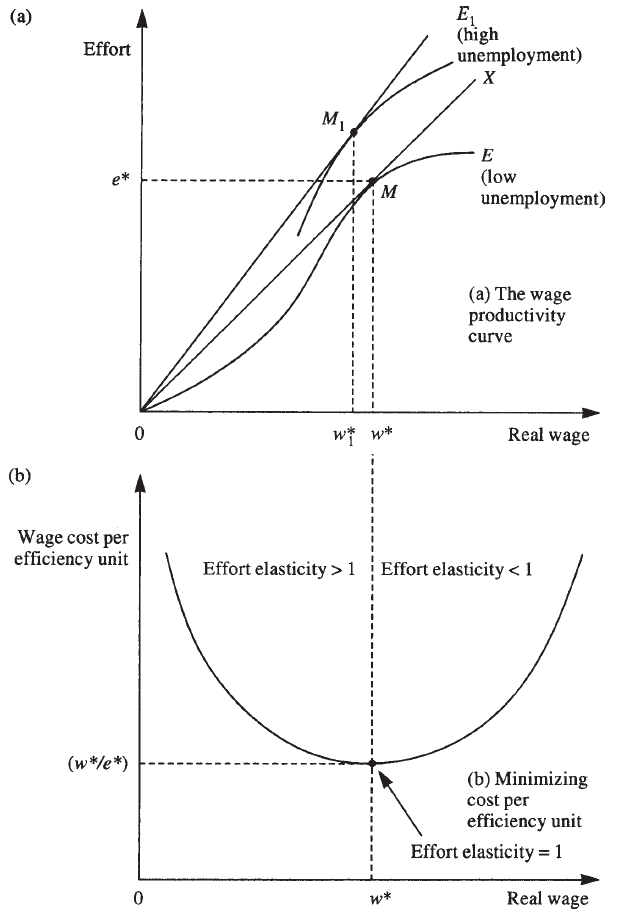
\includegraphics[width=0.3\textwidth]{./figures/aula15_fig6.PNG}}
        \caption{Salário-eficiência e condição de Solow. Fonte: Snowdon e Vane (2005).}
        \label{aula15_fig6}
    \end{figure}
\end{frame}

\begin{frame}{Rigidez de salário real: salário-eficiência}
    \begin{itemize}
        \item Painel (a): curva de esforço mostra relação entre esforço dos trabalhadores e salário real\bigskip
        \item Quanto maior o salário real, maior o esforço dispendido\bigskip
        \item Inicialmente há uma região de retornos crescentes: aumentos no salário real levam a um aumento mais do que proporcional no nível de esforço do trabalho (produtividade)\bigskip
        \item O esforço por unidade monetária pode ser mensurado por $e/w$ e esta razão é maximizada no ponto $M$, onde $0X$ é tangente à função esforço\bigskip
        \item Note que à medida que a inclinação da curva $E$ aumenta, o custo do salário por unidade de eficiência declina\bigskip
        \item Como $e/w$ é maximizado em $M$ a um salário-eficiência $w^*$, o custo salarial por unidade de eficiência também atinge um mínimo ao salário $w^*$
    \end{itemize}
\end{frame}

\begin{frame}{Rigidez de salário real: salário-eficiência}
    \begin{itemize}
        \item Se a firma é capaz de contratar toda a mão-de-obra que desejar ao nível de salário que oferece, irá maximizar seus lucros ao oferecer um salário-eficiência $w^*$ que satisfaça duas condições:\bigskip
        \begin{enumerate}
            \item \textcolor{lightgray}{A elasticidade do esforço com relação ao salário real é unitária (isso significa que a firma deve fixar um salário que minimize os custos do trabalho por unidade de eficiência)}\bigskip
            \item A firma deverá contratar mão-de-obra até o ponto em que o produto marginal do trabalho é igual ao salário-eficiência
        \end{enumerate}
    \end{itemize}
\end{frame}

\begin{frame}{Rigidez de salário real: salário-eficiência}
    \begin{itemize}
        \item Se a demanda agregada por trabalho ao salário $w^*$ é menor que a oferta agregada, teremos desemprego involuntário no equilíbrio de mercado\bigskip
        \item Dado que a taxa salarial ótima $w^*$ independe do nível de emprego ou do parâmetro de produtividade $A$, um choque que desloca a demanda agregada por trabalho induzirá uma variação no nível de emprego mas nenhuma variação no salário real (eficiência) rígido\bigskip
        \item Situação inicial: $D_{L1}$ mostra o produto marginal do trabalho para um dado nível de esforço $e^*$\bigskip
        \item Se o salário-eficiência supera o salário de market-clearing $w^* > w$, então, o equilíbrio de mercado é consistente com desemprego involuntário $U$
    \end{itemize}
\end{frame}

\begin{frame}{Rigidez de salário real: salário-eficiência}
    \begin{figure}
        \centering
        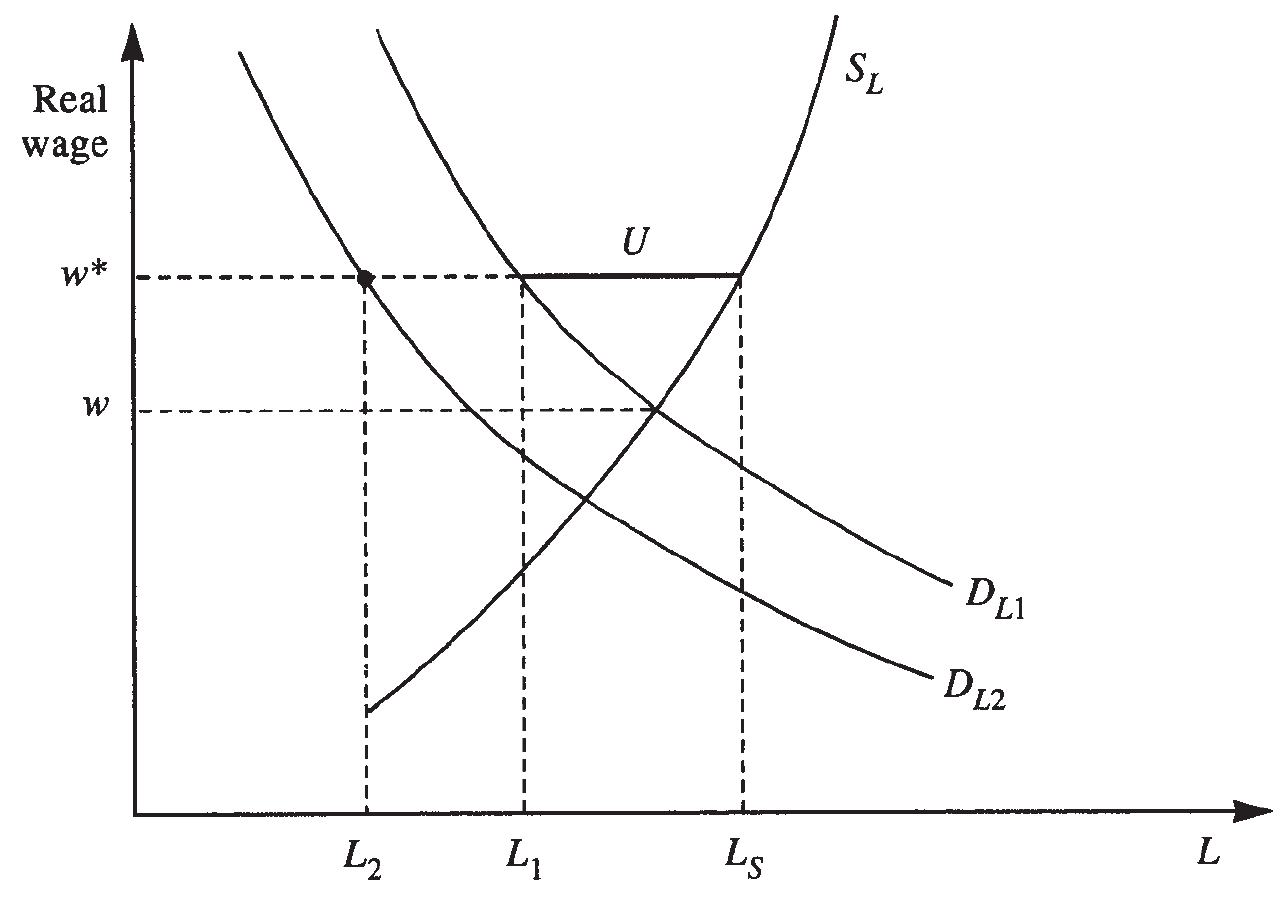
\includegraphics[width=0.6\textwidth]{./figures/aula15_fig7.PNG}
        \caption{Salário-eficiência e desemprego involuntário. Fonte: Snowdon e Vane (2005).}
        \label{aula15_fig7}
    \end{figure}
\end{frame}

\begin{frame}{Rigidez de salário real: salário-eficiência}
    \begin{itemize}
        \item Um choque que desloque a curva de demanda por trabalho para $D_{L2}$ irá aumentar o desemprego involuntário, dado que o salário-eficiência mantém-se em $w^*$\bigskip
        \item Apenas no caso em que o salário de equilíbrio Walrasiano (market-clearing) superar o salário-eficiência que inexistirá desemprego involuntário\bigskip
        \item Com $w > w^*$, firmas são forçadas a pagar o salário Walrasiano\bigskip
        \item No entanto, é provável que $w^* > w$\bigskip
        \item Se um aumento no desemprego influenciar o esforço dos trabalhadores empregados, a curva de esforço se desloca para cima, o que diminui o salário ao qual $e/w$ é maximizado - $w_1^*$ na Figura \ref{aula15_fig6}
    \end{itemize}
\end{frame}

\begin{frame}{Rigidez de salário real: salário-eficiência}
    \begin{itemize}
        \item Por que esforço é relacionado positivamente ao salário real?\bigskip
        \item Economias em desenvolvimento: salários mais altos aumentam o bem-estar físico dos trabalhadores via aumento no consumo de alimentos e melhoria na qualidade da alimentação, e ao reduzir desnutrição salários reais mais altos aumentam a eficiência do trabalho (Leibenstein, 1957; Bardhan, 1993)\bigskip
        \item Em contexto de países desenvolvidos uma outra justificativa é necessária\bigskip
        \item Quatro categorias de teorias de salário-eficiência:\bigskip
        \begin{enumerate}
            \item Modelo de seleção adversa (Weiss, 1980)\bigskip
            \item Modelo de rotatividade de mão-de-obra (labour turnover) (Salop, 1979)\bigskip
            \item Modelo de \emph{shirking} (Shapiro e Stiglitz, 1984)\bigskip
            \item Modelo de \emph{fairness} (Akerlof, 1982)
        \end{enumerate}
    \end{itemize}
\end{frame}

\begin{frame}{Rigidez de salário real: seleção adversa}
    \begin{itemize}
        \item Firmas que oferecem salários mais altos irão atrair melhores trabalhadores\bigskip
        \item Mercado de trabalho habitado por indivíduos heterogêneos, firmas com informação imperfeita acerca das características de produtividade dos candidatos (predomínio de informação assimétrica)\bigskip
        \item Trabalhadores possuem maiores informações sobre suas habilidades, comprometimento, etc. do que empregadores antes de serem contratados e irão sinalizar para potenciais empregadores informações a respeito de suas qualidades (e.g., qualificações, nível de escolaridade, histórico de empregos anteriores, salário atual se empregados)\bigskip
        \item Dada a existência de custos não-negligenciáveis de contratação e demissão, firmas preferem não contratar trabalhadores e demitir funcionários de baixa produtividade\bigskip
        \item Firmas também podem incorrer em elevados custos de treinamento de novos funcionários antes de ficar claro que não "estão à altura"
    \end{itemize}
\end{frame}

\begin{frame}{Rigidez de salário real: seleção adversa}
    \begin{itemize}
        \item Uma forma de evitar este problema é enviar sinalizações ao mercado sob a forma de ofertas de salários elevados\bigskip
        \item Weiss (1980): o salário ofertado por uma firma influencia o número e a qualidade dos candidatos aos postos de trabalho\bigskip
        \item Se as habilidades do trabalhador estão relacionadas aos seus salários de reserva, ofertas salariais mais elevadas irão atrair os candidatos mais produtivos e qualquer candidato que aceitar trabalhar por menos que o salário-eficiência será considerado um possível "limão"\bigskip
        \item Firmas também ficam relutantes em reduzir salários mesmo ao se depararem com um excesso de oferta de mão-de-obra à oferta de salário prevalente\bigskip
        \item Isso acontece pois isso pode induzir os trabalhadores mais produtivos a se demitir voluntariamente
    \end{itemize}
\end{frame}

\begin{frame}{Rigidez de salário real: seleção adversa}
    \begin{itemize}
        \item Como resultado, um equilíbrio de subemprego emergirá\bigskip
        \item Para evitar problemas de seleção adversa, firmas podem introduzir dispositivos de triagem, mas estas mensurações envolvem custos, assim como o monitoramento contínuo dos trabalhadores depois que foram contratados
    \end{itemize}
\end{frame}

\begin{frame}{Rigidez de salário real: rotatividade da mão-de-obra}
    \begin{itemize}
        \item Outra razão para firmas pagarem um salário-eficiência acima do de market-clearing: reduzir rotatividade de mão-de-obra que traz custos consideráveis\bigskip
        \item A disposição de um trabalhador em se demitir diminuirá significativamente se uma firma pagar um salário acima do de equilíbrio de market-clearing\bigskip
        \item Com taxas de demissões sendo uma função decrescente do salário real, firmas têm um incentivo a pagar um salário-eficiência para reduzir rotatividade do trabalho\bigskip
        \item Salop (1979): equilíbrio no mercado de trabalho caracterizado por desemprego involuntário dado que todas as firmas precisam aumentar seus salários para dissuadir trabalhadores que querem se demitir\bigskip
        \item Em situações nas quais o desemprego aumenta, o prêmio salarial necessário para impedir aumento na rotatividade diminuirá
    \end{itemize}
\end{frame}

\begin{frame}{Rigidez de salário real: \emph{shirking}}
    \begin{itemize}
        \item Maioria das atividades: contratos de trabalho são incompletos, o que permite que trabalhadores tenham discrição no que diz respeito ao nível de esforço dispendido\bigskip
        \item Contratos não especificam cada aspecto da performance do trabalhador e de suas atividades\bigskip
        \item Como coletar informações a respeito de trabalhadores individuais e o monitoramento contínuo são custosos para a firma, o pagamento de um salário-eficiência $w^* > w$ pode funcionar como um mecanismo de disciplina para o trabalhador\bigskip
        \item Assimetria de informações: trabalhadores sabem mais sobre seu nível de esforço do que empregadores, isso cria um problema de agente-principal\bigskip
        \item Isso acontece quando o bem-estar do principal é influenciado pela ação (ou inação) do agente
    \end{itemize}
\end{frame}

\begin{frame}{Rigidez de salário real: \emph{shirking}}
    \begin{itemize}
        \item Mercado de trabalho: o principal é o dono da empresa e os gerentes, o agente é o trabalhador\bigskip
        \item A ameaça de demissão não é efetiva em um mercado de trabalho no qual trabalhadores conseguem facilmente encontrar um novo emprego à mesma taxa salarial\bigskip
        \item Se a firma paga um salário acima da concorrência, ou se existe desemprego, trabalhadores tem incentivo a não \emph{shirk}, dado que existe um custo real de demissão e \emph{shirking} torna-se mais arriscado para cada trabalhador\bigskip
        \item Shapiro-Stiglitz (1984): o pagamento de um salário-eficiência age como um desincentivo a \emph{shirking}, desemprego involuntário em equilíbrio é um resultado de problemas que firmas se deparam quando monitoramento é imperfeito 
    \end{itemize}
\end{frame}

\begin{frame}{Rigidez de salário real: \emph{shirking}}
    \NB{
        If it pays one firm to raise its wage it will pay all firms to raise their wages.\bigskip

        \flushright{(Shapiro e Stiglitz, 1984).}\bigskip
    }
    \begin{itemize}
        \item Aumento no nível geral de salários aumenta desemprego, mesmo que todas as firmas paguem o mesmo salário-eficiência, ainda há um desincentivo a \emph{shirking} pois caso seja pego, trabalhador enfrenta possibilidade de desemprego prolongado\bigskip
        \item O 'exército de reserva' age como um mecanismo de desincentivo\bigskip
        \item Portanto, o esforço do trabalhador empregado pela firma $i$ é uma função do tipo:
        \begin{equation}
            e_i = e_i(w_i, w_{-i}, u)
        \end{equation}
        \item Quando $w_i = w_{-i}$, \emph{shirking} depende positivamente do nível de emprego
    \end{itemize}
\end{frame}

\begin{frame}{Rigidez de salário real: \emph{shirking}}
    \begin{figure}
        \centering
        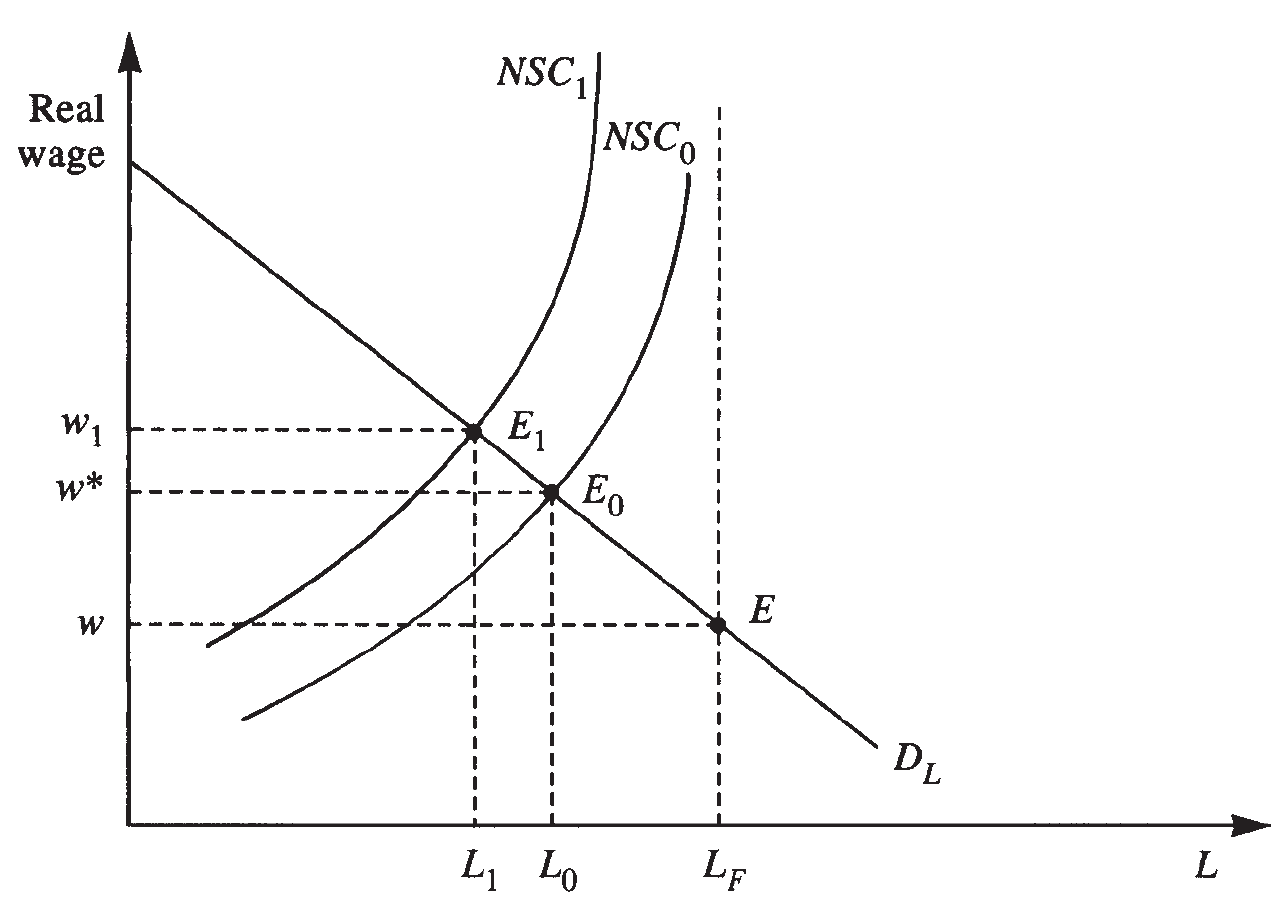
\includegraphics[width=0.6\textwidth]{./figures/aula15_fig8.PNG}
        \caption{Modelo \emph{shirking}. Fonte: Snowdon e Vane (2005).}
        \label{aula15_fig8}
    \end{figure}
\end{frame}

\begin{frame}{Rigidez de salário real: \emph{shirking}}
    \begin{itemize}
        \item A restrição de \emph{no-shirking} (NSC) indica o salário mínimo a cada nível de emprego abaixo do qual acontecerá \emph{shirking}\bigskip
        \item Na figura, o salário de \emph{market-clearing} é $w$\bigskip
        \item Note que \emph{no-shirking} é inconsistente com pleno emprego\bigskip
        \item Incentivo para \emph{no-shirking}: ofertar um salário-eficiência acima de $w$\bigskip
        \item Se todas as firmas ofertam $w^*$, o mecanismo de disciplina será o risco de desemprego
    \end{itemize}
\end{frame}

\begin{frame}{Rigidez de salário real: \emph{shirking}}
    \begin{itemize}
        \item Note que a necessidade de pagar um salário acima de $w$ diminui à medida que o desemprego aumenta\bigskip
        \item Além disso, o salário-eficiência $w^*$ e o nível de emprego $L_0$ estão associados a um nível de desemprego involuntário de equilíbrio indicado por $L_F - L_0$\bigskip
        \item Como NSC está sempre acima e à esquerda da curva de oferta de trabalho, sempre haverá desemprego involuntário no equilíbrio\bigskip
        \item A curva NSC desloca para a esquerda se a firma reduz intensidade de monitoramento e/ou o governo, e.g., aumenta seguro-desemprego\bigskip
        \item Nestes casos, o salário necessário para evitar \emph{shirking} a cada nível de emprego será maior\bigskip
        \item Novo equilíbrio: modelo prevê aumento no salário-eficiência e na taxa de desemprego involuntário de equilíbrio
    \end{itemize}
\end{frame}

\section{Teoria de ciclos}
\begin{frame}{Ciclos econômicos}
    \begin{itemize}
        \item Novos-Keynesianos: choques que geram distúrbios agregados podem ser de lado de oferta ou demanda \bigskip
        \item Existência de fricções e imperfeições que amplificam estes choques, resultando em flutuações consideráveis no produto real e emprego \bigskip
        \item Menor importância para fonte dos choques, questão mais relevante é saber como economia responde a estes choques\bigskip
        \item Duas vertentes:\bigskip
        \begin{enumerate}
            \item Ênfase na importância de rigidezes nominais\bigskip
            \item Explora o impacto potencialmente desestabilizador da flexibilidade de preços e salários (Keynes, 1936 e Tobin, 1975)
        \end{enumerate}
    \end{itemize}    
\end{frame}

% \begin{frame}{\emoji{books} Bibliografia}
%     \begin{itemize}                        
%         \item Solow, R.M. (1998), ‘How Cautious Must the Fed Be?’, in R.M. Solow and J.B. Taylor, Inflation, Unemployment and Monetary Policy, Cambridge, MA: MIT Press\medskip        
%         \item Svensson, L.E.O. (1997), ‘Optimal Inflation Targets, “Conservative” Central Banks and Linear Inflation Contracts’, American Economic Review\medskip
%         \item Taylor, H. (1985), ‘Time Inconsistency: A Potential Problem for Policymakers’, Federal Reserve Bank of Philadelphia Business Review\medskip
%         \item Taylor, J.B. (1980), ‘Aggregate Dynamics and Staggered Contracts’, Journal of Political Economy\medskip
%         \item Waller, C.J. and Walsh, C.E. (1996), ‘Central Bank Independence, Economic Behaviour and Optimal Term Lengths’, American Economic Review\medskip
%         \item Walsh, C.E. (1993), ‘Central Bank Strategies, Credibility and Independence: A Review Essay’, Journal of Monetary Economics\medskip
%         \item Walsh, C.E. (1995), ‘Optimal Contracts for Central Bankers’, American Economic Review\medskip
%     \end{itemize}
% \end{frame}
\end{document}